\subsection*{映像ストリーミング}
全天球映像の送受信にはZoom Video Communicationsの
Zoom\cite{1}を使用した.

\begin{table}[tp]
  \begin{center}
  \begin{tabular}{cc}
  最大解像度 & 1280x720 \\
  最大fps & 30      
  \end{tabular}
  \caption{Zoomの仕様}
  \end{center}
  \end{table}

\subsection*{仮想カメラ}
映像のキャプチャ手段としてOBS Studio\cite{9}を用いている.
OBS Studioは起動中のアプリケーションや画面全体,接続されたカメラ
の映像をキャプチャー・合成して作成した映像をYoutube等の動画配信サイトへ
ストリーミングできるアプリケーションである.
以下の図のタイマーのキャプチャのように,キャプチャしてきたアプリの
映像にエフェクトを加えることも可能である.(映像では青色のクロマキーフィルタを
加え,背景を透明にしている)

\begin{figure}[tp]
  \centering
  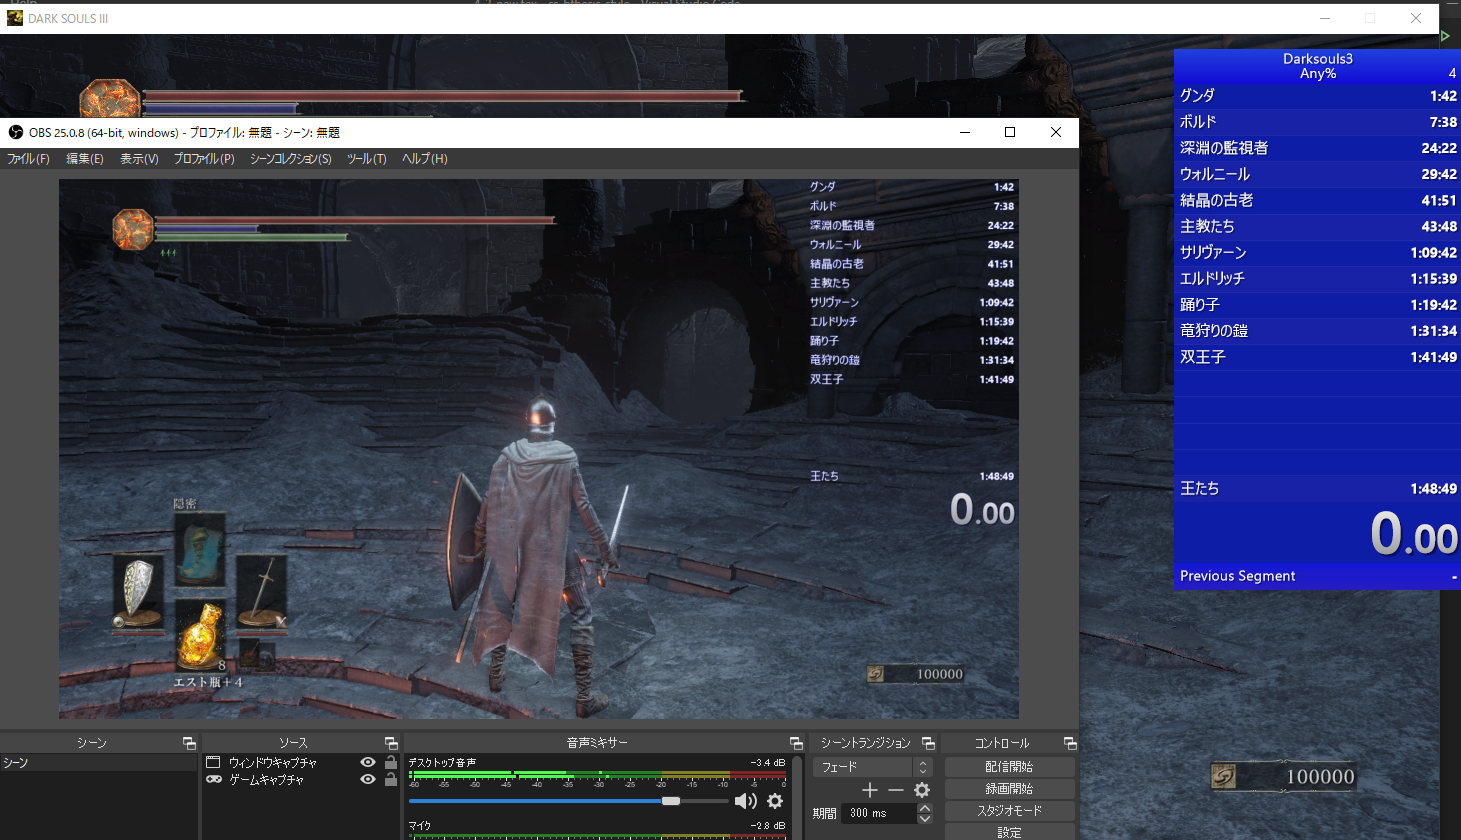
\includegraphics[scale=0.4]{fig/OBSstudio.png}
  \caption{OBSStudioで画面をキャプチャする様子}
\end{figure}

仮想カメラとしては,OBS-virtual-cam\cite{7}を
用いた.この仮想カメラの仕様は以下のようになっている.
 

\begin{table}[tp]
  \begin{center}
  \begin{tabular}{cc}
  最大解像度 & 1280x720 \\
  最大fps & 60      
  \end{tabular}
  \caption{OBS-virtual-camの仕様}
  \end{center}
  \end{table}

OBS-virtual-cameraはOBS Stuioの機能であり,これを用いればOBS Studio
でキャプチャ中の映像を,仮想カメラの映像として扱うことが出来るようになる.
仮想カメラは,他アプリケーションからPCに物理的に付属したカメラと同様に
認識され,ストリーミングや映像の加工などが容易になる.

\begin{figure}[tp]
  \centering
  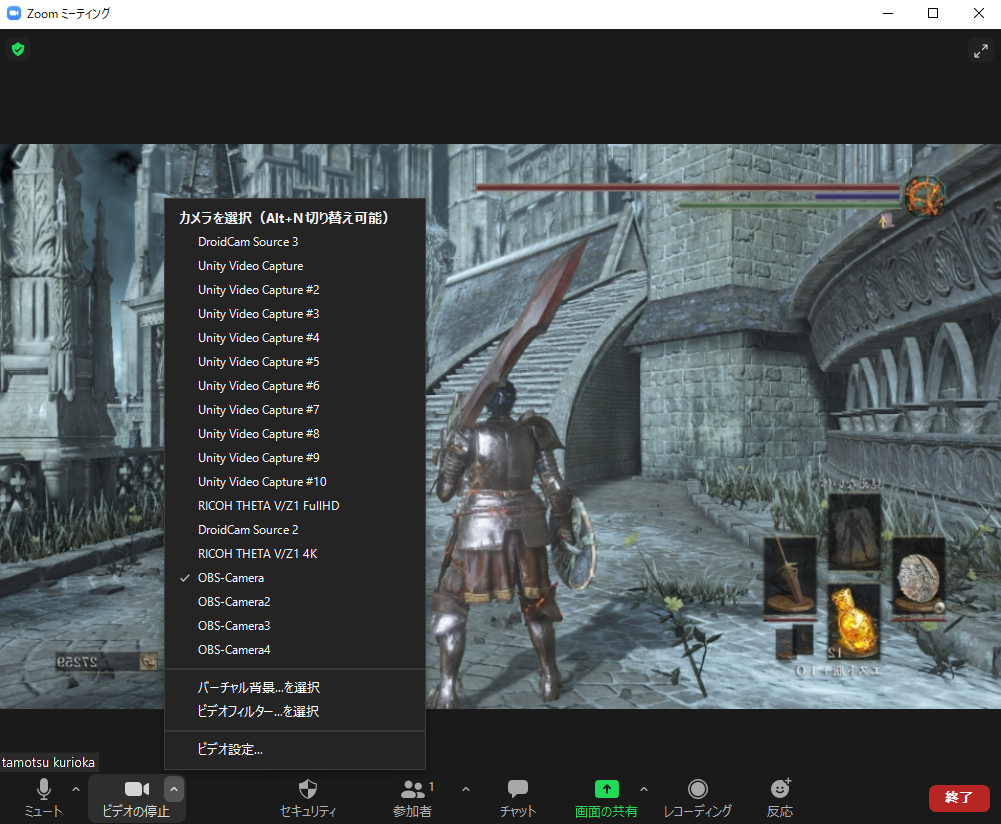
\includegraphics[scale=0.5]{fig/streaming.png}
  \caption{zoomでのOBS-virtual-camの映像ストリーミング}
\end{figure}

\subsection*{映像の加工}
映像の加工には,pythonのライブラリの1つであるOpenCVを用いた.
先述した通り,全天球ビデオカメラのパノラマ映像は正距円筒図法を用いて
出力されている.glomal350を用いる際にはさらに正距方位図法に変換
する必要がある.

\begin{figure}[tp]
  \centering
  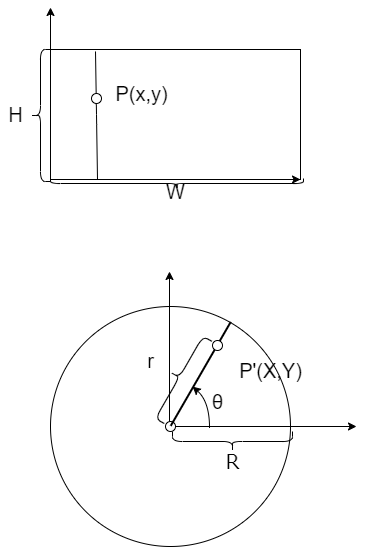
\includegraphics[scale=1.0]{fig/convertintocircle.png}
  \caption{正距円筒図から正距方位図への変換}
\end{figure}

縦$H$,横$W$の大きさで表された正距円筒図の点$P(x,y)$が
半径$R$の正距方位図で点$P'(X,Y)$に写されるとすると,以下の関係式が成り立つ.


\begin{eqnarray}
  \theta = \frac{2\pi x}{W}  \nonumber \\
  r = \frac{Ry}{H} \nonumber \\
  X = r\cos{\theta} \nonumber \\
  Y = r\sin{\theta} \nonumber
\end{eqnarray}

この関係式を用いることで,全天球ビデオカメラで撮影した
パノラマ画像を,glomal350で投影するための正距方位図法を用いた
画像へと変換することが出来る.

\subsection*{GUIの構築}
アプリケーションを操作しやすいようにGUIを構築した.
GUIの構築には,pythonのライブラリであるTkinterを用いた.

Tkinterでは,他のGUIアプリケーション制作ライブラリと同じように,
ボタンや画像などを表示させることが出来るほか,画像にカーソルを重ねたときに
発生するイベント等を登録することができる.今回は,顔をクリックすると
画像が平行移動する処理や,実験の解析のために操作のログを残すために使用した.